\documentclass[uplatex,titlepage]{jsarticle}
% PDFへのリンク付与用
%(ソースコードに対して, 大きく変更を加えてくるスタイルファイルなので, 必ず一番最初に読み込むこと!)
\usepackage[
dvipdfmx,
hidelinks, %リンクを目立たなくする
pdftitle={知識情報処理演習I, IIレポート}, %題目
pdfauthor={17NM708N 鈴木雅也} %著者
]{hyperref}
\usepackage{pxjahyper}

%画像読み込み用
\usepackage[dvipdfmx]{graphicx}
\usepackage[dvipdfmx]{color}

%listings
\usepackage{listings}
\usepackage{jlisting}
\lstset{
language=Java,
frame=Tb, %フレーム
breaklines=true, %行が長くなってしまった場合, 改行する
numbers=left, %左側に行番号表示
basicstyle={\small},
tabsize=2,
showstringspaces=false
}

\title{知識情報処理演習I, IIレポート}
\author{理工学研究科情報工学専攻情報工学コース1年\\17NM708N 鈴木雅也}

\begin{document}
\maketitle
\section{はじめに}
本レポートでは, ゲーム木探索に対する理解を目標にNegaMax法を用いたオセロのプログラムを作成した.

\section{開発環境}
開発環境は表\ref{tab:開発環境}のようになっている. ここでKotlin\footnote{\url{http://kotlinlang.org/}}とはJVM上で動作するプログラミング言語であり, Javaとの互換性を有している.
\begin{table}[h]
\begin{center}
\label{tab:開発環境}
\caption{開発環境}
\begin{tabular}{c|c}
\hline
\hline
OS & Ubuntu 16.04 LTS \\
プログラミング言語 & Kotlin 1.1 \\
JDK & Java SE Development Kit 8 \\
ライブラリ & JavaFX \\
IDE & IntelliJ IDEA Ultimate 2017.2 \\
 & Scene Builder 8.3.0 \\ \hline
\end{tabular}
\end{center}
\end{table}


\section{ディレクトリ構造}
\subsection{リソース}
\begin{itemize}
\item \underline{settings.xml (ソースコード\ref{list:settings.xml})}\\
プログラムの設定
\item \underline{resources.xml (ソースコード\ref{list:resources.xml})}\\
デフォルトのリソース
\item \underline{resources\_ja.xml (ソースコード\ref{list:resources_ja.xml})}\\
日本語用リソース
\end{itemize}

\clearpage
\subsection{プログラム io/github/massongit/othello2017/kotlin/}
\begin{itemize}
\item \underline{main.kt (ソースコード\ref{list:main.kt})}\\
mainメソッド (プログラムの始点)
\end{itemize}

\subsubsection{アプリケーション app/}
\begin{itemize}
\item \underline{MainApplication.kt (ソースコード\ref{list:MainApplication})}\\
GUIの始点 (画面の切り替え等を行う)
\item \underline{DisplayType.kt (ソースコード\ref{list:DisplayType})}\\
画面の種類
\item メニュー画面 menu/
\begin{itemize}
\item \underline{Menu.fxml (ソースコード\ref{list:Menu.fxml})}\\
メニュー画面のView
\item \underline{Menu.css (ソースコード\ref{list:Menu.css})}\\
メニュー画面用CSS
\item \underline{MenuController.kt (ソースコード\ref{list:MenuController})}\\
メニュー画面のController
\end{itemize}
\item スタート画面 start/
\begin{itemize}
\item \underline{StartDisplay.fxml (ソースコード\ref{list:StartDisplay.fxml})}\\
スタート画面のView
\item \underline{StartDisplay.css (ソースコード\ref{list:StartDisplay.css})}\\
スタート画面用CSS
\item \underline{StartDisplayController.kt (ソースコード\ref{list:StartDisplayController})}\\
スタート画面のController
\end{itemize}
\item プレイ画面 play/
\begin{itemize}
\item \underline{Node.kt (ソースコード\ref{list:Node})}\\
ゲームの各ターンに対応したノードの雛形
\item \underline{PlayDisplay.fxml (ソースコード\ref{list:PlayDisplay.fxml})}\\
プレイ画面のView
\item \underline{PlayDisplay.css (ソースコード\ref{list:PlayDisplay.css})}\\
プレイ画面のCSS
\item \underline{PlayDisplayController.kt (ソースコード\ref{list:PlayDisplayController})}\\
プレイ画面のController. ゲームの各ターンに対応したノードの一種として扱われている.
\clearpage
\item 情報パネル information/
\begin{itemize}
\item \underline{Information.fxml (ソースコード\ref{list:Information.fxml})}\\
情報パネルのView
\item \underline{Information.css (ソースコード\ref{list:Information.css})}\\
情報パネルのCSS
\item \underline{InformationController.kt (ソースコード\ref{list:InformationController})}\\
情報パネルのController
\end{itemize}
\item 石 stone/
\begin{itemize}
\item \underline{Stone.kt (ソースコード\ref{list:Stone})}\\
石を表すGUI部品
\item \underline{Move.kt (ソースコード\ref{list:Move})}\\
着手を表すGUI部品. 石の一種として扱われている.
\item \underline{StoneState.kt (ソースコード\ref{list:StoneState})}\\
石の種類
\end{itemize}
\item AI ai/
\begin{itemize}
\item \underline{AI.kt (ソースコード\ref{list:AI})}\\
AIの雛形
\item \underline{AIStrength.kt (ソースコード\ref{list:AIStrength})}\\
AIの強さ
\item ノード node/
\begin{itemize}
\item \underline{AINode.kt (ソースコード\ref{list:AINode})}\\
AIによるゲーム木探索で使用するノードの雛形
\item \underline{AINodeType.kt (ソースコード\ref{list:AINodeType})}\\
AIによるゲーム木探索で使用するノードの種類
\end{itemize}
\item NegaMax法によるAI nega\_max/
\begin{itemize}
\item \underline{NegaMaxAI.kt (ソースコード\ref{list:NegaMaxAI})}\\
NegaMax法によるAI
\item \underline{NegaMaxNode.kt (ソースコード\ref{list:NegaMaxNode})}\\
NegaMax法におけるゲーム木探索で使用するノード
\end{itemize}
\end{itemize}
\end{itemize}
\end{itemize}

\subsubsection{ユーティリティ utils/}
\begin{itemize}
\item \underline{XMLResourceBundleControl.kt (ソースコード\ref{list:XMLResourceBundleControl})}\\
XML形式の設定ファイルに対応したController
\item \underline{big\_integer.kt (ソースコード\ref{list:big_integer.kt})}\\
BigIntegerのビット演算をKotlinのビット演算子と同様に記述できるようにするためのライブラリ
\end{itemize}

\section{実装}
\subsection{盤面処理}
Wikipedia\cite{wikipedia}を参考に, ビット演算による盤面処理の高速化を行った. この際, Kotlinの基本型のひとつであるLong型では盤面全体を表現し切れないため, ビットを扱うオブジェクトとして, Javaの標準ライブラリであるjava.math.BigIntegerを用いている. また, 盤面処理を着手の探索の際に行い, 反転処理ではその結果を用いることで反転処理の高速化を行っている.

\subsection{AI}
次の2種類のAIを実装した. なお. AIに人間らしさを出すため, AIの思考時間を実際の思考時間より300〜1199ms程度長く取っている.
\begin{itemize}
\item \underline{強いAI}\\
ユーザがどんなに強くても勝ちに行くことを目指したAI. Negamax法と$\beta$カットを用い, 10手先まで読む. 葉ノードにおける着手の数を$x$, 葉ノードの子ノードにおける着手の数をそれぞれ$y_1, y_2, ..., y_n$としたとき, 評価関数は次のようになる.
\begin{equation}
x+\max(-y_1, -y_2, ..., -y_n)
\end{equation}
\item \underline{弱いAI}\\
ユーザがどんなに弱くても負けに行くことを目指したAI. 強いAIをベースに, 次のような変更を加えた.
\begin{itemize}
\item 最大値を取る箇所で最小値を取る
\item $\beta$カットの代わりに$\alpha$カットを用いる
\end{itemize}
\end{itemize}

\clearpage
\section{スクリーンショット}
\begin{figure}[h]
\begin{center}
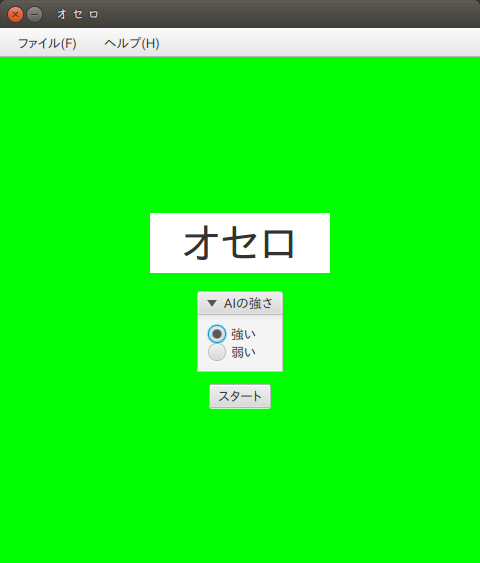
\includegraphics[scale=0.5]{オセロ_036}
\caption{スタート画面}
\end{center}
\end{figure}
\begin{figure}[h]
\begin{center}
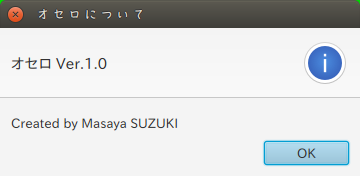
\includegraphics[scale=0.5]{オセロについて_037}
\caption{バージョン情報の表示}
\end{center}
\end{figure}
\begin{figure}[h]
\begin{center}
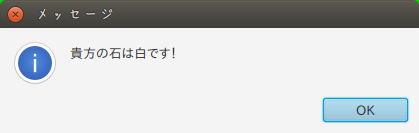
\includegraphics[scale=0.5]{メッセージ_038}
\caption{先手後手の表示}
\end{center}
\end{figure}
\begin{figure}[h]
\begin{center}
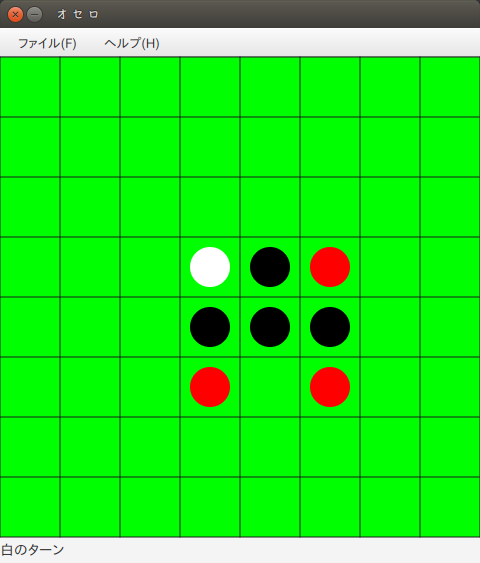
\includegraphics[scale=0.5]{オセロ_039}
\caption{プレイ画面}
\end{center}
\end{figure}
\begin{figure}[h]
\begin{center}
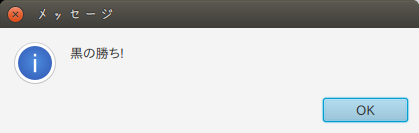
\includegraphics[scale=0.5]{メッセージ_036}
\caption{勝敗の表示}
\end{center}
\end{figure}
\begin{figure}[h]
\begin{center}
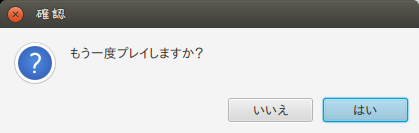
\includegraphics[scale=0.5]{確認_037}
\caption{もう一度プレイするかどうかの選択}
\end{center}
\end{figure}

\clearpage
\section{考察}
強いAIにおいては, 一般に不利になると言われている端よりひとつ内側のマスをユーザに取らせようとする傾向があり, 弱いAIにおいては, 一般に有利になると言われている端のマスをユーザに取らせようとする傾向があった. このことから, AIが意図した通りの動作を行っていることがわかった.

\section{まとめ}
本レポートでは, ゲーム木探索に対する理解を目標にNegaMax法を用いたオセロのプログラムを作成した. 実際の実装を通して, NegaMax法や$\alpha$カットや$\beta$カット, 盤面処理といったゲーム木探索で用いられるアルゴリズムやテクニックを理解することができたことから, ゲーム木探索に対する理解という目標は達成できたと考えられる.

\appendix
%参考文献
\bibliography{report}
\bibliographystyle{junsrt}

\section{ソースコード}
\lstinputlisting[caption=settings.xml, label=list:settings.xml]{../resources/settings.xml}
\lstinputlisting[caption=resources.xml, label=list:resources.xml]{../resources/resources.xml}
\lstinputlisting[caption=resources\_ja.xml, label=list:resources_ja.xml]{../resources/resources_ja.xml}
\lstinputlisting[caption=io/github/massongit/othello2017/kotlin/main.kt, label=list:main.kt]{../src/io/github/massongit/othello2017/kotlin/main.kt}
\lstinputlisting[caption=io.github.massongit.othello2017.kotlin.app.MainApplication, label=list:MainApplication]{../src/io/github/massongit/othello2017/kotlin/app/MainApplication.kt}
\lstinputlisting[caption=io.github.massongit.othello2017.kotlin.app.DisplayType, label=list:DisplayType]{../src/io/github/massongit/othello2017/kotlin/app/DisplayType.kt}
\lstinputlisting[caption=io/github/massongit/othello2017/kotlin/app/menu/Menu.fxml, label=list:Menu.fxml]{../src/io/github/massongit/othello2017/kotlin/app/menu/Menu.fxml}
\lstinputlisting[caption=io/github/massongit/othello2017/kotlin/app/menu/Menu.css, label=list:Menu.css]{../src/io/github/massongit/othello2017/kotlin/app/menu/Menu.css}
\lstinputlisting[caption=io.github.massongit.othello2017.kotlin.app.menu.MenuController, label=list:MenuController]{../src/io/github/massongit/othello2017/kotlin/app/menu/MenuController.kt}
\lstinputlisting[caption=io/github/massongit/othello2017/kotlin/app/start/StartDisplay.fxml, label=list:StartDisplay.fxml]{../src/io/github/massongit/othello2017/kotlin/app/start/StartDisplay.fxml}
\lstinputlisting[caption=io/github/massongit/othello2017/kotlin/app/start/StartDisplay.css, label=list:StartDisplay.css]{../src/io/github/massongit/othello2017/kotlin/app/start/StartDisplay.css}
\lstinputlisting[caption=io.github.massongit.othello2017.kotlin.app.start.StartDisplayController, label=list:StartDisplayController]{../src/io/github/massongit/othello2017/kotlin/app/start/StartDisplayController.kt}
\lstinputlisting[caption=io.github.massongit.othello2017.kotlin.app.play.Node, label=list:Node]{../src/io/github/massongit/othello2017/kotlin/app/play/Node.kt}
\lstinputlisting[caption=io/github/massongit/othello2017/kotlin/app/play/PlayDisplay.fxml, label=list:PlayDisplay.fxml]{../src/io/github/massongit/othello2017/kotlin/app/play/PlayDisplay.fxml}
\lstinputlisting[caption=io/github/massongit/othello2017/kotlin/app/play/PlayDisplay.css, label=list:PlayDisplay.css]{../src/io/github/massongit/othello2017/kotlin/app/play/PlayDisplay.css}
\lstinputlisting[caption=io.github.massongit.othello2017.kotlin.app.play.PlayDisplayController, label=list:PlayDisplayController]{../src/io/github/massongit/othello2017/kotlin/app/play/PlayDisplayController.kt}
\lstinputlisting[caption=io/github/massongit/othello2017/kotlin/app/play/information/Information.fxml, label=list:Information.fxml]{../src/io/github/massongit/othello2017/kotlin/app/play/information/Information.fxml}
\lstinputlisting[caption=io/github/massongit/othello2017/kotlin/app/play/information/Information.css, label=list:Information.css]{../src/io/github/massongit/othello2017/kotlin/app/play/information/Information.css}
\lstinputlisting[caption=io.github.massongit.othello2017.kotlin.app.play.information.InformationController, label=list:InformationController]{../src/io/github/massongit/othello2017/kotlin/app/play/information/InformationController.kt}
\lstinputlisting[caption=io.github.massongit.othello2017.kotlin.app.play.stone.Stone, label=list:Stone]{../src/io/github/massongit/othello2017/kotlin/app/play/stone/Stone.kt}
\lstinputlisting[caption=io.github.massongit.othello2017.kotlin.app.play.stone.Move, label=list:Move]{../src/io/github/massongit/othello2017/kotlin/app/play/stone/Move.kt}
\lstinputlisting[caption=io.github.massongit.othello2017.kotlin.app.play.stone.StoneState, label=list:StoneState]{../src/io/github/massongit/othello2017/kotlin/app/play/stone/StoneState.kt}
\lstinputlisting[caption=io.github.massongit.othello2017.kotlin.app.play.ai.AI, label=list:AI]{../src/io/github/massongit/othello2017/kotlin/app/play/ai/AI.kt}
\lstinputlisting[caption=io.github.massongit.othello2017.kotlin.app.play.ai.AIStrength, label=list:AIStrength]{../src/io/github/massongit/othello2017/kotlin/app/play/ai/AIStrength.kt}
\lstinputlisting[caption=io.github.massongit.othello2017.kotlin.app.play.ai.node.AINode, label=list:AINode]{../src/io/github/massongit/othello2017/kotlin/app/play/ai/node/AINode.kt}
\lstinputlisting[caption=io.github.massongit.othello2017.kotlin.app.play.ai.node.AINodeType, label=list:AINodeType]{../src/io/github/massongit/othello2017/kotlin/app/play/ai/node/AINodeType.kt}
\lstinputlisting[caption=io.github.massongit.othello2017.kotlin.app.play.ai.nega\_max.NegaMaxAI, label=list:NegaMaxAI]{../src/io/github/massongit/othello2017/kotlin/app/play/ai/nega_max/NegaMaxAI.kt}
\lstinputlisting[caption=io.github.massongit.othello2017.kotlin.app.play.ai.nega\_max.NegaMaxNode, label=list:NegaMaxNode]{../src/io/github/massongit/othello2017/kotlin/app/play/ai/nega_max/NegaMaxNode.kt}
\lstinputlisting[caption=io.github.massongit.othello2017.kotlin.utils.XMLResourceBundleControl, label=list:XMLResourceBundleControl]{../src/io/github/massongit/othello2017/kotlin/utils/XMLResourceBundleControl.kt}
\lstinputlisting[caption=io/github/massongit/othello2017/kotlin/utils/big\_integer.kt, label=list:big_integer.kt]{../src/io/github/massongit/othello2017/kotlin/utils/big_integer.kt}
\end{document}
